\chapter{\label{chp:createframework}Creating the framework}
\section{Create new project}
To create a new project, the directory hierarchy needs to be copied from a source to the destination, and directories and filenames need to be altered to match the design name. Filelist and setting files also needs to be altered to include the correct design file names. This process is automated into a bash script, \textit{CreateNewProject.sh}. To run the script, the directory \textit{\_source}, containing the source project, must be present in the directory where the script is run.

The directory- and file-tree of the framework is shown in \cref{fig:frameworkdirtree}. Directories are colored cyan, executables and scripts are colored teal, and other design and constraint files are colored violet. File comment or description are in black. Each file is described in the comment on the right side. 
\begin{figure}
\centering

\begin{minipage}{0.99\textwidth}
    \renewcommand*\DTstyle{\sffamily\tiny}
    \dirtree{%
    .1 \textcolor{cyan}{\slash}.
    .2 \textcolor{cyan}{\_source}.
    .3 \textcolor{cyan}{ip}.
    .4 \textcolor{cyan}{designname}.
    .5 \textcolor{cyan}{hls}.
    .6 \textcolor{teal}{constraintsGenerator{.}run} \dotfill \:\:\begin{minipage}[t]{5.4cm}
                                                    Program to generate constraint and Makefiles
                                                    \end{minipage}.
    .6 \textcolor{violet}{constraints{.}xlsx} \dotfill \:\:\begin{minipage}[t]{5.4cm}
                                                            Setup-file for constraint-generator
                                                            \end{minipage}. 
    .5 \textcolor{cyan}{lay}.
    .6 \textcolor{teal}{Makefile} \dotfill \:\:\begin{minipage}[t]{5.4cm}
                                                    Makefile for running layout
                                                    \end{minipage}.
    .5 \textcolor{cyan}{pow}.
    .6 \textcolor{teal}{Makefile} \dotfill \:\:\begin{minipage}[t]{5.4cm}
                                                    Makefile for running power analysis
                                                    \end{minipage}.
    .6 \textcolor{teal}{power\_analysis{.}tcl} \dotfill \:\:\begin{minipage}[t]{5.4cm}
                                                    Settings file for power analysis
                                                    \end{minipage}.
    .5 \textcolor{cyan}{rtl}.
    .6 \textcolor{violet}{designname{.}fl} \dotfill \:\:\begin{minipage}[t]{5.4cm}
                                                    Filelist specifying files in the design
                                                    \end{minipage}.
    .6 \textcolor{violet}{designname{.}v} \dotfill \:\:\begin{minipage}[t]{5.4cm}
                                                    Verilog designfile generated by LegUp
                                                    \end{minipage}.
    .5 \textcolor{cyan}{sim}.
    .6 \textcolor{cyan}{run}.
    .7 \textcolor{violet}{designname{.}args} \dotfill \:\:\begin{minipage}[t]{5.4cm}
                                                            Argument simulation tool
                                                            \end{minipage}.
    .7 \textcolor{violet}{designname{.}comp} \dotfill \:\:\begin{minipage}[t]{5.4cm}
                                                            Compilation parameter file for simulation{.} Specifies filelist for design and testbench{.}
                                                            \end{minipage}.
    .7 \textcolor{violet}{designname{.}sim} \dotfill \:\:\begin{minipage}[t]{5.4cm}
                                                            Simulation parameter file for simulation{.} Specifies top-level testbench module and simulation options{.}
                                                            \end{minipage}.
    .7 \textcolor{violet}{modelsim{.}ini} \dotfill \:\:\begin{minipage}[t]{5.4cm}
                                                            Settings-file for simulation tool
                                                            \end{minipage}.
    .7 \textcolor{teal}{RUN\_ALL} \dotfill \:\:\begin{minipage}[t]{5.4cm}
                                                            Script to run simulation
                                                            \end{minipage}.
    .6 \textcolor{cyan}{tb}.
    .7 \textcolor{violet}{test\_designname{.}fl} \dotfill \:\:\begin{minipage}[t]{5.4cm}
                                                    Filelist specifying files in testbench
                                                    \end{minipage}.
    .7 \textcolor{violet}{test\_designname{.}v} \dotfill \:\:\begin{minipage}[t]{5.4cm}
                                                    Verilog testbench file generated by LegUp
                                                    \end{minipage}.
    .7 \textcolor{violet}{test\_designname\_testcases{.}v} \dotfill \:\:\begin{minipage}[t]{5.4cm}
                                                    File containing testcases to be included in testbench generation in LegUp
                                                    \end{minipage}.
    .5 \textcolor{cyan}{syn}.
    .6 \textcolor{cyan}{dc\_scripts}.
    .7 \textcolor{violet}{designname{.}constraints{.}tcl} \dotfill \:\:\begin{minipage}[t]{5.4cm}
                                                            Synthesis constraint file{.} Clocks are specified here{.}
                                                            \end{minipage}.
    .6 \textcolor{violet}{common\_setup{.}tcl} \dotfill \:\:\begin{minipage}[t]{5.4cm}
                                                            Setup file for synthesis 
                                                            \end{minipage}.
    .6 \textcolor{teal}{Makefile} \dotfill \:\:\begin{minipage}[t]{5.4cm}
                                                            Makefile for running synthesis
                                                            \end{minipage}.
    .5 \textcolor{violet}{designname{.}c} \dotfill \:\:\begin{minipage}[t]{5.4cm}
                                                            C file for functions design specification
                                                            \end{minipage}.
    .5 \textcolor{teal}{HLSScript{.}sh} \dotfill \:\:\begin{minipage}[t]{5.4cm}
                                                            Script for running framework
                                                            \end{minipage}. 
    .5 \textcolor{teal}{Makefile} \dotfill \:\:\begin{minipage}[t]{5.4cm}
                                                            Makefile for running tool-flow without framework/HLS
                                                            \end{minipage}. 
    .5 \textcolor{violet}{results{.}xlsx} \dotfill \:\:\begin{minipage}[t]{5.4cm}
                                                            File to visualize and compare framework results
                                                            \end{minipage}. 
    .3 \textcolor{cyan}{methodology} \dotfill \:\:\begin{minipage}[t]{5.4cm}
                                                            Scripts and utilities for toolchain
                                                            \end{minipage}. 
    .2 \textcolor{teal}{CreateNewProject{.}sh} \dotfill \:\:\begin{minipage}[t]{5.4cm}
                                                            Script for creating new project
                                                            \end{minipage}. 
    }
\end{minipage}
\caption{Directory and file-tree of the framework}
\label{fig:frameworkdirtree}
\end{figure}
The script manages the whole process of copying and renaming files, and replacing the correct strings in the setting files and scripts. When run, the script asks for the name of the new project, and replaces any occurrences of the word \textit{designname} in the \textit{\_source}-directory with the given name. The user does not need to change any of the scripts or Makefiles, only update design specific files as described in \cref{sec:runframework}.

\section{\label{sec:hlsscript}Framework-script}
To automate the process of generating multiple design in LegUp and running of the tool-flow on the generated designs, a script is created. LegUp is running on a VirtualBox image and not on the same servers where the rest of the tool-flow are located. This means that some files and commands must be transferred between different machines. In \cite{holm2015pro}, a possible solution using SSH and SCP was proposed. The script is built on this method, but first some additional preparations needs to be made. Since the VirtualBox guest is running on a local computer, a port forwarding rule has to be added to allow connections to port 22 of the guest from the Linux servers of Nordic Semiconductor. The connections has to go through the host computer, as the VirtualBox guest does not have any direct connection to the network. The setting can either be set using the GUI of VirtualBox, or by running the following command from a command line:
\begin{verbatim}
  VBoxManage modifyvm myserver --natpf1 "ssh,tcp,,3022,,22"  
\end{verbatim}
Here \textit{myserver} is the name of the VirtualBox VM and should be replaced with the name used when the LegUp image was added in VirtualBox. When this setting is added, it is possible to establish a connection over SSH from the Linux server directly to LegUp by connecting to the port 3022 and the local IP-address of the computer running VirtualBox.

The standard SSH and SCP packages on Linux systems does not support passing the password as an argument to the command. To avoid the need to enter username and password each time a file is transferred using SCP, or a command is executed using SSH, it is necessary to setup key-based authentication. This can be done manually, but the framework-script can also do this setup automatically if you pass the flag \textit{-s}. What the script does, is to generate a RSA key-file for the current user with \textit{ssh-keygen} and copy the generated file to LegUp using \textit{ssh-copy-id}. The password is passed to \textit{ssh-copy-id} using \textit{spawn}, \textit{expect} and \textit{send} commands.

The script has seven main tasks:
\begin{enumerate}
    \item Generate constraint and Makefiles
    \item Run \gls{hls}-tool to generate Verilog design and testbench files
    \item Run simulation
    \item Run synthesis
    \item Run layout
    \item Run power analysis
    \item Collect relevant parameters from reports and generate readable result files.
\end{enumerate}
The five tasks in the middle are mostly transferring of files to and from LegUp, and running make-commands. These steps use the tool-flow described in \cref{sec:toolflowbg}. The first and last task are a bit more comprehensive, and is described in the following two subsections. When the script is finished generating and running the tool-flow on one design, the directories \textit{rtl}, \textit{sim}, \textit{syn}, \textit{lay}, and \textit{pow} is copied into a directory named with the designnumber under the \textit{hls}-directory. The script is written for the bash-shell, and the full code of the script is listed in \cref{sec:hlsscriptsourcecode}.

\subsection{Constraint generating}
In order to run \gls{hls} with a variety of different constraints and settings, one constraint and one Makefile need to be generated for each run. To automate this process, an Excel document, \textit{constraints.xlsx}, has been created. Sheet 2 of this document, shown in \cref{fig:excelconstraintssetup}, contains the setup of the constraints. Here the user can select which constraints should be randomized and also set if the constraint should have a specific value. Some values are required, and must have the value specified. If a parameter is not needed, the user can specify that the default value of the parameter should be kept. 
\begin{figure}[hbpt]
\centering
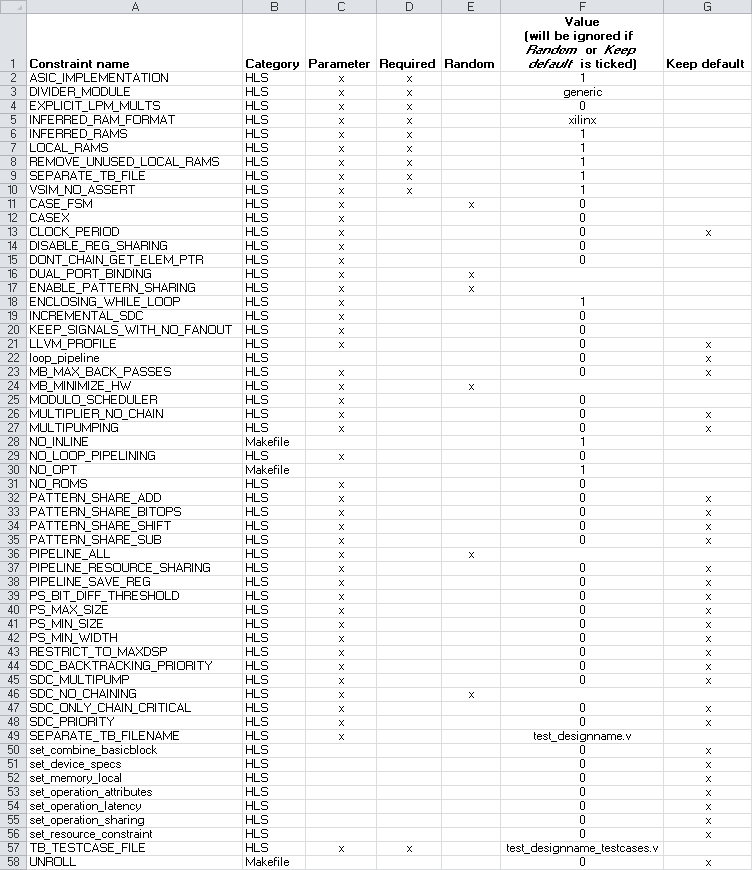
\includegraphics[width=\textwidth]{../figs/ConstraintGenerationSetup.png}
\caption{\label{fig:excelconstraintssetup}Setup of constraint file generation in Excel spreadsheet}
\end{figure}
Sheet 1 of the Excel file contains a \gls{csv} format of the constraint settings. The format of one \gls{csv}-string is:
\begin{verbatim}
parameterName,value,required,random,parameter,makefile,keepDefault
\end{verbatim}
Only the fields relevant for the parameter will be printed to the \gls{csv}, for instance the parameter \textit{CASE\_FSM} will print the line "\verb!CASE_FSM,random,parameter!", as this is the relevant fields for this parameter given the setup of the spreadsheet. Similar, the parameter \textit{NO\_OPT} will print the line "\verb!NO_OPT,1,makefile!", since this is a Makefile-parameter defined to have the value 1. The \gls{csv} format is copied from the Excel-file to a \gls{csv} file by using the headless tool \textit{convert-to} in libreoffice, with the command "\verb!libreoffice --headless --convert-to csv!". The \gls{csv}-file can then be read by the program generating constraint- and Makefiles. 

The program \textit{constraintGenerator.run} takes the filename of the \gls{csv}-file, the level parameter for the Makefile, and the designname as inputs, and returns the number of generated constraint files. This number is used in the framework-script to run the framework the correct number of times. This program is also written in the language C++, with reasoning similar to the one explained in \cref{subsec:llvmirparserprogram}. By parsing through the above described \gls{csv}-file, the program generate one constraint file and accompanying Makefile for each variation of the randomized constraint-parameters. Currently only parameters taking a 1-bit binary value is supported by the constraint generator program. This gives a total of $2^N$ designs, where \textit{N} is the number of randomized parameters. The constraints is set using a binary counter, meaning that for 3 randomized parameters, the first constraint file will have the values 0,0,0, the second file 0,0,1, the third file 0,1,0, and so on. The generated constraint and Makefiles are output to the directories \textit{constraintfiles} and \textit{makefiles} under the \textit{hls}-directory. The full code of the program generating constraint and Makefiles are listed in \cref{sec:constraintgeneratorsourcecode}.

\subsection{Report generating}
As the framework-script can be used to generate a large amount of designs, it is important to easily be able to collect the important data from all the generated reports. To ease the process of data collecting, the script collects the data from all designs and stores it in separate files. The data is collected using \textit{grep} commands, and the data is stripped of unnecessary text, using bash's substring replacement function, before output to files. The collected data is stored under the \textit{reports}-directory, with the file-names:
\begin{multicols}{2}
\textbf{From synthesis:}\\
\verb!register_count.rpt!

\textbf{From Layout:}\\
\verb!combinational_area.rpt!\\
\verb!noncombinational_area.rpt!\\
\verb!design_area.rpt!

\textbf{From power analysis:}\\
\verb!net_switching_power.rpt!\\
\verb!cell_internal_power.rpt!\\
\verb!cell_leakage_power.rpt!\\
\verb!total_power.rpt!

\textbf{Combined:}\\
\verb!all_results.rpt!
\end{multicols}

Each file contains the information specified by the filename. The corresponding design number is not included in the files, but the first line of each file contain results from design 0, the second line contain results from design 1, and so on. In the reports from power analysis, 5 values is stored at each line of the file, separated by commas. This is because the power analysis run five different power scenarios, each generating one result. The other files only contain a single value at each line. To simplify the process of importing the data into spreadsheets or other visualization-tools all files are joined horizontally into a single file, \textit{all\_results.rpt}. This means that each line will contain all values for a single design. The values in this file will be separated by tabs. This tidy file can be imported in Excel or other tools for generating graphs or compare data. Comparison could be made automatic if desired, but this is not implemented at this stage.

\section{\label{sec:runframework}Running the framework}
Before running the framework, some files need to be changed. The functional specification needs to be added to the file \textit{designName.c} and testcases for the simulation can be added to the file \textit{test\_designName\_testcases.v} under the directory \textit{sim/tb/}. In addition, the desired constraints need to be selected or filled out in the file \textit{constraints.xlsx} in the \textit{hls}-directory. To run the framework, the file \textit{HLSScript.sh} is executed from a shell. Depending on the design size, available licences, and number of randomized constraints, the run-time of the framework can be long. If the framework seems stuck on one of the tasks, check the log file, \textit{HLSscript.log}, for errors.

